\section{Data Sources}\label{sec:source}

Previous surveys~\cite{Tao2005, Zhang2014, Poria2017, Garcia2017} put forward that different data sources should be applied to various modeling methods in multimodal affective computing. Poria et al.~\cite{Poria2017} also give the argument that 90\% literature consider visual, audio and text information as multimodal affect analysis instead of other dimensions by their extensive literature review.

In this section, we discuss the commonly existing data sources in a typical smartphone and prepare for the modelling method in the next section. Figure~\ref{fig:source} illustrates the data flow from sensors to user emotion state.

\begin{figure}
    \centering
    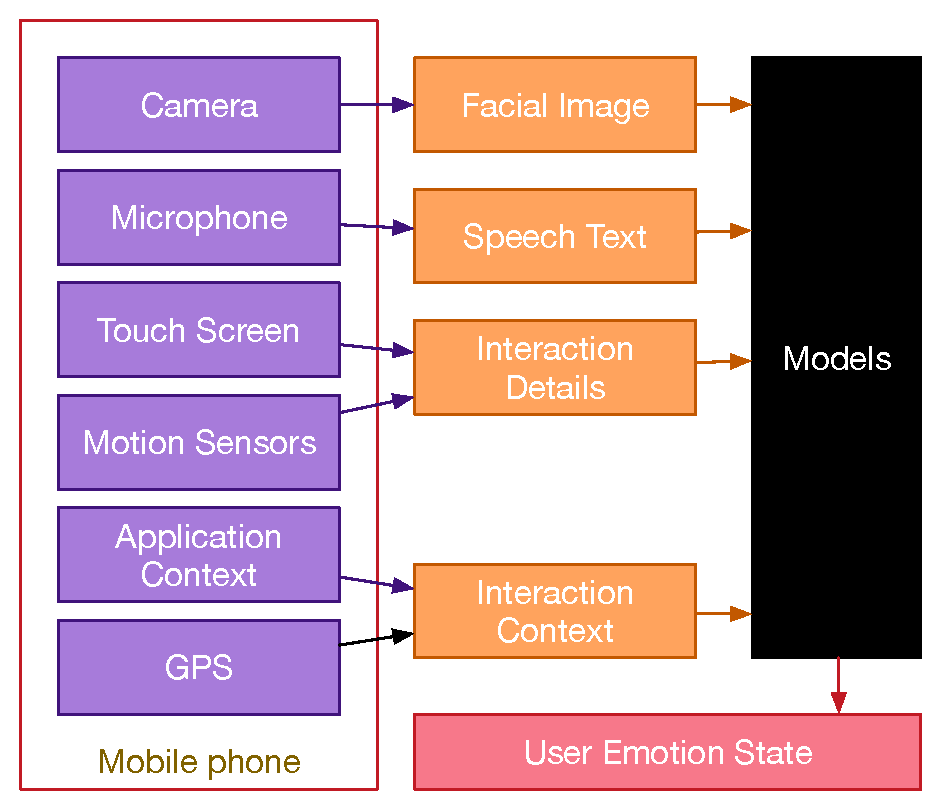
\includegraphics[width=0.5\textwidth]{source}
    \caption{Data sources can be used in emotion inference which provided by the most of commercial mobile phone devices.}
    \label{fig:source}
\end{figure}

\subsection{Camera}\label{subsec:vision}
We emphasise vision sensors in the first place since face and facial expressions are undoubtedly one of the most critical nonverbal channels used by humans to convey internal emotion~\cite{james2013emotion, Poria2017}. This part mainly discusses vision sensors, which includes RGB cameras and depth cameras, and illustrates how vision sensors can be used for affective emotion inference.

Pure RGB cameras have been widely used in a commercial smartphone as an image sensor. 
For the camera with depth information on mobile devices (recently introduced TrueDepth Camera in iPhone X, see Figure~\ref{fig:ipx}\footnote{\url{https://www.apple.com/iphone-x/\#truedepth-camera}}) combines infrared camera, flood illuminator, proximity sensor, ambient light sensor, front-facing camera and dot projector to provide depth images of facial information of a user.

\begin{figure}
    \centering
    \label{fig:ipx}
    \includegraphics[width=0.5\textwidth]{ipx}
    \caption{TrueDepth Camera in iPhone X}
\end{figure}

\subsection{Microphone}\label{subsec:audio}
Audio sensors usually refer to built-in microphones; they collect voice information from current environments, which can infer user emotions based on their speech content.

Before recognizing user speech, a system usually should take care and preprocess the environmental noise and detect acoustic fingerprint~\cite{boles2017voice} (i.e., voiceprint) for the current user, isolate their speech from mixed audio information.

Inferring emotions from user speech can be split into two parts; The first part is recognizing the speech text from the user~\cite{mikolov2010recurrent, google2017}, then understanding or inference from the text, namely sentiment analysis~\cite{Rajalakshmi2017ACS}.

\subsection{Touch Screen}\label{subsec:touch}

Human emotions can be expressed in different ways. Emotional communication has focused predominantly on the facial and vocal channels but has ignored the tactile channel~\cite{hertenstein2009communication}, researchers investigated the possible expressions of user emotion in detail while they are using mobile devices with touch screen.

A capacitive touch screen provides touch position, touch pressure, touch angle through time. Among the subsequent researches~\cite{Gao2012, Shah2015, Mottelson2016, bhattacharya2017predictive}, researchers explored how human emotions can be inferred by capacitive touch channel in a specific application context based on these features. This is typically done only with touch screen interface.

Interestingly, 3D touch screen was largely introduced in commercial devices a few years ago. Some of the researches investigated the possibility of haptic based application~\cite{Eid2016}. Mazzoni~\cite{Mazzoni2016} and Lentini~\cite{Lentini2017} showed how a system with haptic touch response essentially can express and influence user emotions. Bhattacharya~\cite{Bhattacharya2017} concludes that haptic-based affect detection remains an understudied topic.

\subsection{Motion Sensors}\label{subsec:motion}

Motion sensors typically combine gyroscope and accelerometer, which are yet another interaction detail information~\cite{Zhang2014}. An accelerometer measures proper acceleration (acceleration it experiences relative to free fall), felt by people or objects. Most smartphone accelerometers trade large value range for high precision. The gyroscope can be a handy tool in peculiar ways and defines gravity. Gyroscopes have been around for a century, and they are now used everywhere from airplanes, toy helicopters to smartphones. A gyroscope allows a smartphone to measure and maintain orientation. Gyroscopic sensors can monitor and control device positions, orientation, direction, angular motion, and rotation. Figure~\ref{fig:motion} shows the coordinates information of accelerometer and gyroscope sensors.

With these motion sensors, interaction details information such as device holding posture, device moving trajectory can be inferred from these sensor data \cite{Mottelson2016, Poria2017}.

\begin{figure}
    \centering
    \includegraphics[width=0.24\textwidth]{coordinate}
    \includegraphics[width=0.24\textwidth]{coordinate2}
    \caption{Coordinates information of Accelerometer (left) and gyroscope (right) as motion sensors in iOS CoreMotion framework.}
    \label{fig:motion}
\end{figure}

\subsection{GPS}\label{subsec:gps}

GPS sensors provide geographical information of a user, and detect the location of the smartphone using 1) GPS~\cite{tan2013connectivity}; 2) Laceration/Triangulation of cell towers or wifi networks (with a database of known locations for towers and networks)~\cite{rana2015opportunistic}; 3) Location of an associated cell tower or WiFi networks~\cite{Politou2017}.

However, GPS will not work indoors and can quickly kill the battery. Smartphones can try to automatically select best-suited alternative location provider (GPS, cell towers, WiFi), mostly based on desired precision. With the location, we can study the relationship between life patterns and affective states. For example, most people in playground feel happy while most feel sad in a cemetery.

The location provides additional information to verify the subjective report from participants of affective studies. It may also help to build a confidence mechanism \cite{tan2013connectivity} for subjective reports. Attaching the location to the subjective report would produce confident weights to measure the significance of collected subjective reports. For example, a participant reported that he was happy in a cemetery. But, in common sense, people in the cemetery would be sad. Thus, we could set a low weight as a confidence value to the report, or ask the user is indeed either choosed a right option or not.

\subsection{Application Context}\label{subsec:ui}

As we slightly mentioned in the previous section, most of the mobile affective inference techniques based on a touch screen and motion sensors\cite{Gao2012, Shah2015, Mottelson2016, bhattacharya2017predictive} are based on specific application context, for example, application user interface. This kind of information can be another confidence mechanism in a inference system. Vice versa, the inference systems are only modeling for a specific context. However, this could be a drawback of multimodal emotion inference since a complete system will integrate more models for emotion inference.